%%%%%%%%%%%%%%%%%%%%%%%%%%%%%%%%%%%%%%%%%
% Jacobs Landscape Poster
% LaTeX Template
% Version 1.1 (14/06/14)
%
% Created by:
% Computational Physics and Biophysics Group, Jacobs University
% https://teamwork.jacobs-university.de:8443/confluence/display/CoPandBiG/LaTeX+Poster
% 
% Further modified by:
% Nathaniel Johnston (nathaniel@njohnston.ca)
%
% This template has been downloaded from:
% http://www.LaTeXTemplates.com
%
% License:
% CC BY-NC-SA 3.0 (http://creativecommons.org/licenses/by-nc-sa/3.0/)
%
%%%%%%%%%%%%%%%%%%%%%%%%%%%%%%%%%%%%%%%%%

%----------------------------------------------------------------------------------------
%	PACKAGES AND OTHER DOCUMENT CONFIGURATIONS
%----------------------------------------------------------------------------------------

\documentclass[final]{beamer}
\newcommand{\softmax}{\mathrm{softmax}}
\newcommand{\sigmoid}{\mathrm{sigmoid}}
\DeclareMathOperator*{\argmax}{arg\,max}
\DeclareMathOperator*{\argmin}{arg\,min}
\usepackage{amsmath}
\usepackage[scale=1.24]{beamerposter} % Use the beamerposter package for laying out the poster
\usepackage{tabularx}
    \newcolumntype{L}{>{\raggedright\arraybackslash}X}

\usetheme{confposter} % Use the confposter theme supplied with this template

\setbeamercolor{block title}{fg=ngreen,bg=white} % Colors of the block titles
\setbeamercolor{block body}{fg=black,bg=white} % Colors of the body of blocks
\setbeamercolor{block alerted title}{fg=white,bg=dblue!70} % Colors of the highlighted block titles
\setbeamercolor{block alerted body}{fg=black,bg=dblue!10} % Colors of the body of highlighted blocks
% Many more colors are available for use in beamerthemeconfposter.sty

%-----------------------------------------------------------
% Define the column widths and overall poster size
% To set effective sepwid, onecolwid and twocolwid values, first choose how many columns you want and how much separation you want between columns
% In this template, the separation width chosen is 0.024 of the paper width and a 4-column layout
% onecolwid should therefore be (1-(# of columns+1)*sepwid)/# of columns e.g. (1-(4+1)*0.024)/4 = 0.22
% Set twocolwid to be (2*onecolwid)+sepwid = 0.464
% Set threecolwid to be (3*onecolwid)+2*sepwid = 0.708

\newlength{\sepwid}
\newlength{\onecolwid}
\newlength{\twocolwid}
\newlength{\threecolwid}
\setlength{\paperwidth}{48in} % A0 width: 46.8in
\setlength{\paperheight}{36in} % A0 height: 33.1in
\setlength{\sepwid}{0.024\paperwidth} % Separation width (white space) between columns
\setlength{\onecolwid}{0.22\paperwidth} % Width of one column
\setlength{\twocolwid}{0.464\paperwidth} % Width of two columns
\setlength{\threecolwid}{0.708\paperwidth} % Width of three columns
\setlength{\topmargin}{-0.5in} % Reduce the top margin size
%-----------------------------------------------------------

\usepackage{graphicx}  % Required for including images

\usepackage{booktabs} % Top and bottom rules for tables

%----------------------------------------------------------------------------------------
%	TITLE SECTION 
%----------------------------------------------------------------------------------------

\title{Boosting many low capacity classifiers compared to boosting fewer high capacity classifiers in a context of multiclass classifications} % Poster title

\author{Jonathan Guymont, Marzieh Mehdizad, L\'ea Ricard, Jeff Sylvestre Decary \& Joseph D. Viviano} % Author(s)

\institute{Universit\'e de Montr\'eal and Polytechnique Montr\'eal} % Institution(s)


%----------------------------------------------------------------------------------------

\begin{document}

\addtobeamertemplate{block end}{}{\vspace*{2ex}} % White space under blocks
\addtobeamertemplate{block alerted end}{}{\vspace*{2ex}} % White space under highlighted (alert) blocks

\setlength{\belowcaptionskip}{2ex} % White space under figures
\setlength\belowdisplayshortskip{2ex} % White space under equations

\begin{frame}[t] % The whole poster is enclosed in one beamer frame

\begin{columns}[t] % The whole poster consists of three major columns, the second of which is split into two columns twice - the [t] option aligns each column's content to the top

\begin{column}{\sepwid}\end{column} % Empty spacer column

\begin{column}{\onecolwid} % The first column



%----------------------------------------------------------------------------------------
%	INTRODUCTION
%----------------------------------------------------------------------------------------

\begin{block}{Introduction}

\begin{itemize}
    \item Investigate whether there is any benefit to using Adaboost while keeping ensemble capacity fixed.
    \item Compare models in the same family: a single strong learner, or multiple weaker learners such that the number of trained parameters remains roughly the same. 
    \item Test our hypothesize that using more learners with lower individual capacity will outperform a single learner with equivalent capacity.
\end{itemize}
\end{block}


%\begin{figure}
%
\includegraphics[width=0.8\linewidth]{placeholder.jpg}
%\caption{Figure caption}
%\end{figure}

%----------------------------------------------------------------------------------------
%	Algorithms
%----------------------------------------------------------------------------------------
\begin{block}{Algorithms}
%The three model families we compare are Decision Trees, Logistic Regression and Multi-layer Perceptron (MLP). All boosted ensembles were created with Adaboost. The capacity of Logistic Regression was not controlled and will serve as our baseline.
\textbf{Decision Tree.} Let $d$ be the number of features. At a particular node of the tree, $\sqrt{d}$ features were randomly selected to be tested. At each node, the data is split according to (\ref{eq:tree_obj}).
\begin{equation}
    \theta_m = \argmax_{\theta} H(D_m)-H(D_m|\theta)
    \label{eq:tree_obj}
\end{equation}
Each node is divided in two child until either the maximal depth of the tree $\mathcal{T}$ is reached or the minimum number of sample at a node $\min_{sample}$ is reached. $\mathcal{T}$ and $\min_{sample}$ are two hyperparameters that we used to control the capacity.

\textbf{Logistic Regression.}
\begin{equation}
     p(y=k|\mathbf{x}) = \frac{
     e^{
     \mathbf{W}_{k, \cdot}\mathbf{x}+\mathbf{b}_k
     }
     }
     {
     \sum_{i=1}^m e^{
     \mathbf{W}_{i, \cdot}\mathbf{x}+\mathbf{b}_i
     }
     }
\end{equation}
\textbf{Multi-Layer Perceptrons.}
\begin{equation}
    \begin{split}
        \mathbf{h} = \sigma(\mathbf{W}^{(1)}\mathbf{x} + \mathbf{b}^{(1)}),~~~
        \mathbf{y} = \softmax(\mathbf{W}^{(2)}\mathbf{h} + \mathbf{b}^{(2)}) 
    \end{split}
    \label{eq:mlp}
\end{equation}
We change the dimension of $\mathbf{W}^{(1)}$ and $\mathbf{W}^{(2)}$ (i.e. the size of the hidden layer) to vary the capacity.
\end{block}

\begin{block}{Datasets}

\begin{itemize}
    \item \textbf{Wine Quality}: Using 12 quality features measured from white and red wine, predict how these wines are rated by experts (5 classes).
    \item \textbf{Balanced Forest Cover Type}: Using cartographic variables, predict the correct forest cover type (7 classes).
\end{itemize}

\end{block}


\end{column} % End of the first column

\begin{column}{\sepwid}\end{column} % Empty spacer column

\begin{column}{\twocolwid} % Begin a column which is two columns wide (column 2)

\begin{columns}[t,totalwidth=\twocolwid] % Split up the two columns wide column

\begin{column}{\onecolwid}\vspace{-.6in} % The first column within column 2 (column 2.1)

%----------------------------------------------------------------------------------------
%	Methodology
%----------------------------------------------------------------------------------------

\begin{block}{Methodology}

\textbf{Data pre-processing}: All data was normalized before training. For the wine quality data set, the extremely poor and good wines were merged (respectively) as those classes were very rare. 

\textbf{Hyper-parameter search}: We used the training set to learn the parameters of the model and the validation set to do hyper-parameter selection using randomized search with 50 iterations, and 10 folds inner-loop cross validation. 

\textbf{Performance evaluation}: We used macro $F_1$ score for both hyperparameter tuning and test-set reporting due to unbalanced classes.

\textbf{Capacity variation}: We decrease the capacity of decision tree by reducing the maximum depth of the tree and MLP model by reducing the number of hidden units while proportionally-increasing the number of classifiers.

\end{block}

%----------------------------------------------------------------------------------------

\end{column} % End of column 2.1

\begin{column}{\onecolwid}\vspace{-.6in} % The second column within column 2 (column 2.2)


\begin{block}{Decision Trees Results}
\begin{figure} [H]
    \centering
    \begin{tabular}{cccc}
    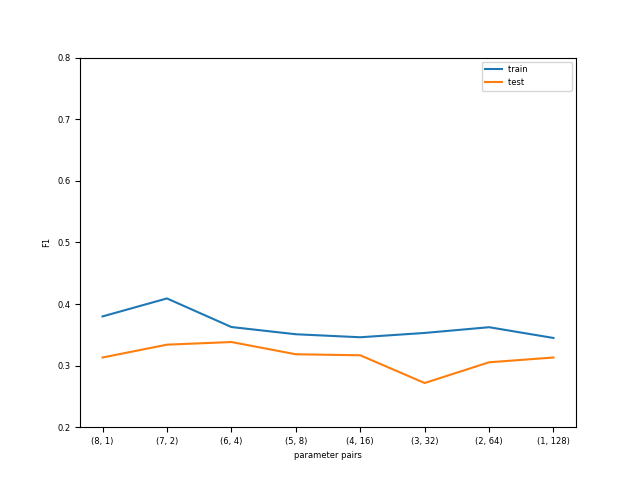
\includegraphics[width=0.5\textwidth]{tree-wine-boosted_f1.png} &
    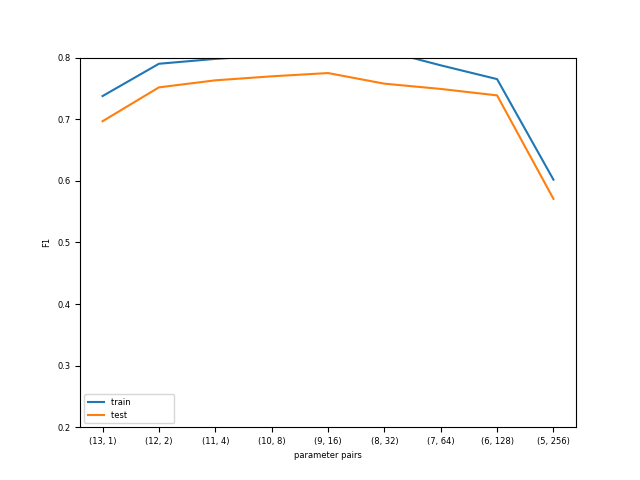
\includegraphics[width=0.5\textwidth]{tree-covtype_balanced-boosted_f1.png}\\
    (a) &
    (b)  \\[6pt]
    \end{tabular}
    \caption{Performance on test and training set by parameter pairs (tree maximum depth, number of tree boosted) on (a) Wine Quality data and (b) Forest Cover Type boosted with Decision Tree classifiers}
    \label{fig:Tree_results}
\end{figure}

\begin{itemize}
    \item The individual capactiy / number of learner tradeoff showed \textbf{no difference between model performance in most cases}.
    \item \textbf{Not a precise method for controlling the number of parameters}, may explain drop in performance with very shallow trees.
\end{itemize}

\end{block}
\end{column} % End of column 2.2
\end{columns} % End of the split of column 2 - any content after this will now take up 2 columns width

%----------------------------------------------------------------------------------------
%	IMPORTANT RESULT
%----------------------------------------------------------------------------------------

%\begin{alertblock}{Important Result}

%Lorem ipsum dolor \textbf{sit amet}, consectetur adipiscing elit. Sed commodo molestie porta. Sed ultrices scelerisque sapien ac commodo. Donec ut volutpat elit.

%\end{alertblock} 

%----------------------------------------------------------------------------------------

\begin{columns}[t,totalwidth=\twocolwid] % Split up the two columns wide column again

\begin{column}{\onecolwid} % The first column within column 2 (column 2.1)


\begin{block}{Logistic Regression Results}
\begin{figure} [H]
    \centering
    \begin{tabular}{cccc}
    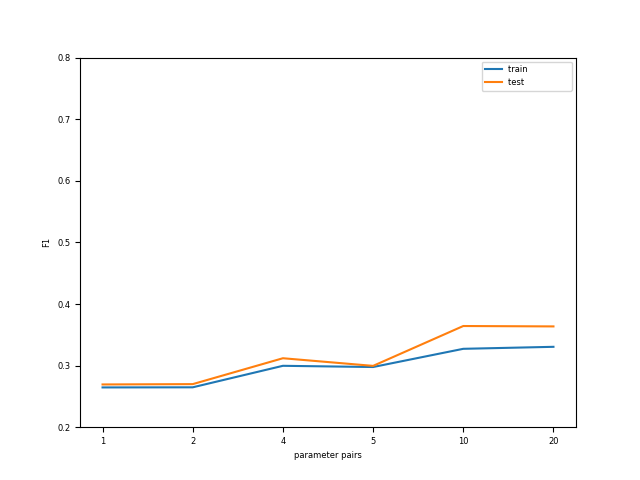
\includegraphics[width=0.5\textwidth]{lr-wine-boosted_f1.png}
    & 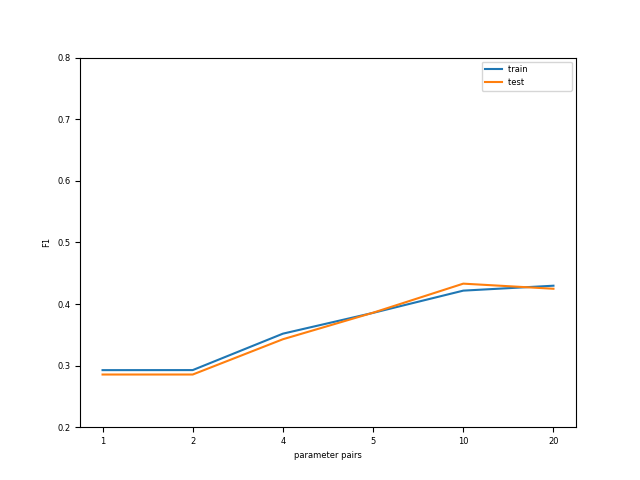
\includegraphics[width=0.5\textwidth]{lr-covtype-boosted_f1.png} \\
    (a) & (b)  \\[6pt]
    \end{tabular}
    \caption{Performance on test and training set by parameter pairs (tree maximum depth, number of tree boosted) on (a) Wine Quality data and (b) Forest Cover Type boosted with Logistic Regression classifiers}
    \label{fig:lr_results}
\end{figure}

\begin{itemize}
    \item \textbf{Adding more learners increases classification performance} for both datasets in the absence of capacity reduction.
    \item Neither model shows evidence of overfitting.
\end{itemize}

\end{block}
\end{column} % End of column 2.1

\begin{column}{\onecolwid} % The second column within column 2 (column 2.2)

%----------------------------------------------------------------------------------------
%	MLP RESULTS
%----------------------------------------------------------------------------------------

\begin{block}{Multi-Layer Perceptrons Results}

\begin{figure} [H]
    \centering
    \begin{tabular}{cccc}
    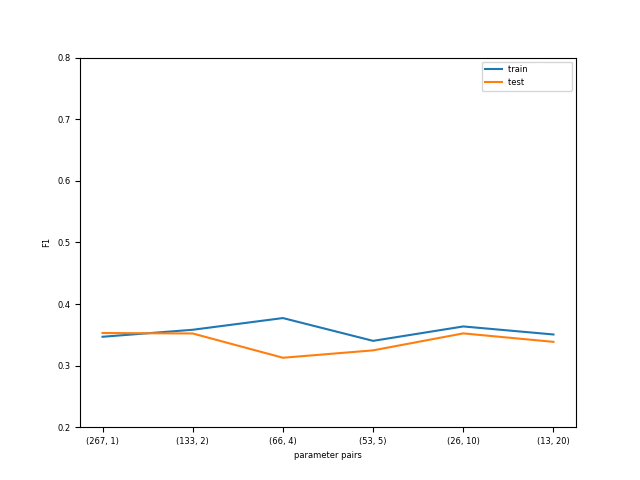
\includegraphics[width=0.5\textwidth]{mlp-wine-boosted_f1.png}
    & 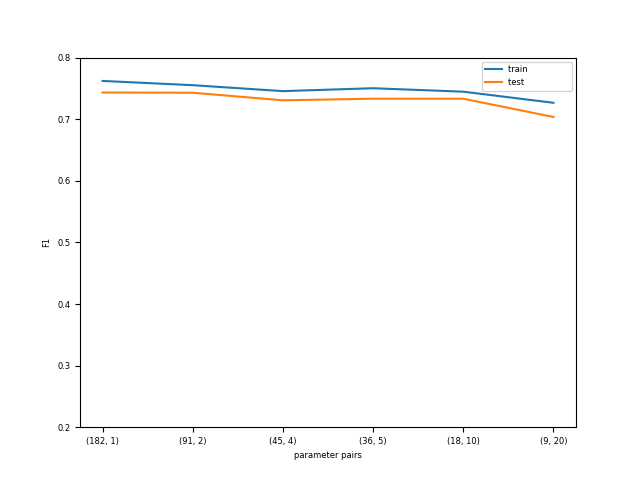
\includegraphics[width=0.5\textwidth]{mlp-covtype_balanced-boosted_f1.png} \\
    (a) & (b)\\[6pt]
    \end{tabular}
    \caption{Performance on test and training set by parameter pairs (number of neurons, number of MLP boosted) on (a) Wine Quality data and (b) Forest Cover Type boosted with MLP classifiers}
    \label{fig:MLP_results}
\end{figure}

\begin{itemize}
    \item When reducing the capacity of the model and proportionally adding more learners, we observe \textbf{no differences in model performance}.
    \item  Easier to \textbf{precisely control the number of parameters} in the model via the hidden layer size.
\end{itemize}

\end{block}

%----------------------------------------------------------------------------------------

\end{column} % End of column 2.2

\end{columns} % End of the split of column 2

\end{column} % End of the second column

\begin{column}{\sepwid}\end{column} % Empty spacer column

\begin{column}{\onecolwid} % The third column

%----------------------------------------------------------------------------------------
%	DISCUSSION
%----------------------------------------------------------------------------------------
\begin{block}{Results Summary}

\begin{table}[h!]
    \begin{center}
    \caption {Test performance of models on Wine Quality}
    \vspace{-65pt}
    \begin{tabular}{|l|l|l|l|l|l|l|}
        \hline
        \multicolumn{7}{|c|}{Wine Quality (boosted)}\\
        \hline
        &\multicolumn{2}{|c|}{Best result}&\multicolumn{2}{|c|}{Highly boosted }&\multicolumn{2}{|c|}{Not boosted}\\
        \hline
        Model & Param. & $F_1$ & Param. & $F_1$ & Param. & $F_1$ \\
        \hline \hline
         LR & (-,10) & 0.36 & (-,20) & 0.36 & (-,1) & 0.26 \\
         Dec. Tree & (6,4) & 0.34 & (1,128) & 0.32 & (8,1) & 0.32 \\
         MLP  & (133,2) & 0.35 & (13,20) & 0.34 & (267,1) & 0.35 \\
         \hline
    \end{tabular}
    \end{center}
    \label{table:Results_Wine}
\end{table}


\begin{table}[h!]
    \caption {Test performance of models on Forest Cover Type }
    \vspace{-65pt}
    \begin{center}
    \begin{tabular}{|l|l|l|l|l|l|l|}
        \hline
        \multicolumn{7}{|c|}{Forest Cover Type (boosted)}\\
        \hline
        &\multicolumn{2}{|c|}{Best result}&\multicolumn{2}{|c|}{Highly boosted}&\multicolumn{2}{|c|}{Not boosted}\\
        \hline
        Model & Param. & $F_1$ & Param. & $F_1$ & Param. & $F_1$ \\
        \hline \hline
         LR & (-,10) & 0.43 & (-,20) & 0.42 & (-,1) & 0.29 \\
         Dec. Tree & (11,64) & 0.53 & (10,128) & 0.51 & (17,1) & 0.41 \\
         MLP  & (91,2) & 0.74 & (9,20) & 0.70 & (182,1) & 0.74 \\
         \hline
    \end{tabular}
    \end{center}
    \label{Table:Results_Forest}
\end{table}

\end{block}

\begin{block}{Discussion and Conclusion}

\begin{itemize}
    \item Adding more classifiers to balance out the loss of per-model capacity recovers the capacity of the stronger individual model model.
    \item Could repeat experiments to obtain good confidence intervals on the $F_1$ scores.
    \item Could compare bagging and boosting methods for datasets with noisy labels (wine dataset) \cite{Diet}.
    \item Evaluating the red and white datasets separately as the features may not correspond across classes.
\end{itemize}

\end{block}

\begin{block}{References}
\begin{thebibliography}{99}
    \bibitem{Diet} Dietterich, T. (2000). An Experimental Comparison of Three Methods for Constructing Ensembles of Decision Trees: Bagging, Boosting, and Randomization. Mach. Learn.. 40. 10.1023
\end{thebibliography}

% \nocite{*} % Insert publications even if they are not cited in the poster
% \small{\bibliographystyle{unsrt}
% \bibliography{sample}\vspace{0.75in}}

\end{block}

%----------------------------------------------------------------------------------------
%	OTHER
%----------------------------------------------------------------------------------------

\setbeamercolor{block title}{fg=red,bg=white} % Change the block title color


\setbeamercolor{block alerted title}{fg=black,bg=norange} % Change the alert block title colors
\setbeamercolor{block alerted body}{fg=black,bg=white} % Change the alert block body colors

%\begin{alertblock}{Contact Information}

%\begin{itemize}
%\item Web: \href{http://www.university.edu/s%\item Email: \href{mailto:john@smith.com}{john@smith.com}
%\item Phone: +1 (000) 111 1111
%\end{itemize}

%\end{alertblock}

\begin{center}
\begin{tabular}{ccc}

\includegraphics[width=0.4\linewidth]{Udem.png} & \hfill &  
\includegraphics[width=0.4\linewidth]{Poly.png}
\end{tabular}
\end{center}

\end{column} % End of the third column
\end{columns} % End of all the columns in the poster
\end{frame} % End of the enclosing frame
\end{document}
